\chapter{Kinematics in Two Dimensions}
	\section{Introduction}
	
	When an object is moving in two (or three) dimensions at once - like when it moves both horizontally and vertically at the same time - the motion of the object in each dimension is completely independent.  This means that each dimension will have its own set of kinematic variables.  The only kinematic variable that can be used in all directions is time, since time is a scalar and does not have a direction.  Thus, instead of only five kinematic variables, problems will have sets of five variables in each direction, with time counting for every dimension.  
	
	
{\renewcommand{\arraystretch}{1.2}
\begin{center}
	
	
	\begin{table}[ht]\caption{\textbf{Kinematic Variables in Multiple Dimensions}}% title of Table 
		\centering % used for centering table	
		\begin{tabular}{|c|c||c|c|}
			\hline \hline
			\textbf{Quantity} & \textbf{Variable} & \textbf{Quantity} & \textbf{Variable}  \\
			\hline
			Horizontal Displacement & $\vec{d_x}$ or $\vec{x}-\vec{x_0}$  & Vertical Displacement & $\vec{d_y}$ or $\vec{y}-\vec{y_0}$ \\
			\hline
		
			Horizontal Initial Velocity & $\vec{v_{ix}}$ or $\vec{v_{0x}}$  & Vertical Initial Velocity & $\vec{v_{iy}}$ or $\vec{v_{0y}}$ \\
\hline

			Horizontal Final Velocity & $\vec{v_{fx}}$ or $\vec{v_x}$  & Vertical Final Velocity & $ \vec{v_{fy}}$ or $\vec{v_y}$ \\ 
	\hline
	Horizontal Acceleration & $\vec{a_x}$  &  Vertical Acceleration & $\vec{a_y} $ \\
	\hline
	\multicolumn{2}{|c|}{Time} & \multicolumn{2}{|c|}{$t$} \\
	\hline
		
		\end{tabular}
		\label{table:kinematic2d}% is used to refer this table in the text
	\end{table}
\end{center}

\section{Projectiles}
\index{Projectiles}

A \textbf{projectile} is any object that meets the following critera:
\begin{itemize}
	\item The object is in \textit{free-fall}.  That is, Gravity is the only force that acts on the object (all other forces are negligable).
	\item The object is moving in two dimensions at the same time.  Most often, describe it as moving both horizontally and vertically at the same time.  
\end{itemize}


\subsection{Horizontally Launched Projectiles}
	\index{Projectiles, Launched Horizontally}
Often, projectiles will be launched horizontally, such as when a ball rolls off a table, or when an archer shoots a perfectly level arrow.  In this case, the math is somewhat easier to deal with.  The initial velocity stated in the problem will be entirely horizontal, and the initial vertical velocity will be zero.


\begin{mdframed}[backgroundcolor=blue!10!white]
	\begin{center}
		
		
		\textbf{Example \thesection.1}	
	\end{center}
	
	\textbf{Problem: } A ball is rolling 2.1 m/s when it rolls off the edge of a 1.3 meter high table.
	\begin{enumerate}
		\item How long is the ball in the air?
		\item How far, horizontally, does the ball land from the edge of the table?
		\item What is the magnitude of the final velocity of the ball?
		\item What is the angle of impact?
	\end{enumerate}
	\vspace{0.1in}
	
	\textbf{Solution:} 
	Begin by drawing a diagram:
	
	\begin{tikzpicture}
		% Draw the table
		%\draw[thick] (0,0) rectangle (1,-1.3);
		%\node at (0.5, -1.4) [below] {Table (1.3 m)};
		
		% Draw the ball's initial position
		\filldraw[black] (0.5,0) circle (0.1);
		%\node at (0.4, 0) [left] {Ball};
		
		% Draw the trajectory of the ball
		\draw[->, thick, dashed] (0.5,0) .. controls (3.5,-1) and (5,-2.5) .. (6,-3.3);
		
		 Draw initial velocity components
		\draw[->, thick, red] (0.5,0) -- (2,0);
		\node at (1.25,0) [above,red] {$v_{0} = 2.1\, \text{m/s}$};
		
		% Draw initial downward velocity
		%\draw[->, thick, blue] (0.5,0) -- (0.5,-0.8);
		%\node at (0.5,-0.4) [left] {$v_y = 0\, \text{m/s}$};
		
		% Draw horizontal and vertical distance markers
		\draw[|-|] (6,0) -- (6,-3.3);
		\node at (6.6,-1.65) [right] {$y-y_0 = \SI{1.3} {m}$};
		
		\draw[|-|] (0.5,-3.3) -- (6,-3.3);
		\node at (3.25,-3.6) [below] {$x-x_0$};
		
		%Draw the coordinate system
			\draw[->,blue] (-1.5,1) -- (-1.5,0.5);
		\node at (-1.5,0.4) [below,blue] {+y};
		
			\draw[->,blue] (-1.5,1) -- (-1,1);
			\node at (-0.9,1) [right,blue] {+x};

		
		% Final velocity and angle markers
		%\draw[->, thick, green] (6,-3.3) -- (6.5,-4);
		%\node at (6.5,-3.6) [right] {$\vec{v}$};
		
		%\draw[->] (6,-3.3) -- (7,-3.3);
		%\node at (7,-3.3) [above] {$v_x$};
		
		%\draw[->] (6,-3.3) -- (6,-4.5);
		%\node at (6,-4.5) [left] {$v_y$};
		
		% Draw angle of impact
		%\draw (6,-3.3) arc[start angle=-90, end angle=-60, radius=1];
		%\node at (6.8,-3.8) {$\theta$};
		
	\end{tikzpicture}
	
	You may notice from the coordinate system that the downward direction has been chosen as +y.  This will help us to avoid needing negatives in the problem.
	
	Next, we create a table with each of the kinematic variables for each dimension:
	
	\begin{longtable}{|c l | c l|}
		\hline
		\multicolumn{2}{|c|}{\textbf{Horizontal}} & \multicolumn{2}{|c|}{\textbf{ Vertical}} \\
		\hline
		$\vec{x}-\vec{x_0}$ =&     & $\vec{y}-\vec{y_0} = $ & $\SI{1.3}{m}$ \\
		\hline
		$\vec{v_{0x}} = $ & $\SI{2.1}{m/s}$ & $\vec{v_{0y}} = $ & $\SI{0}{m/s}$ \\
		\hline
		$v_x = $&  & $v_y = $ &  \\
		\hline
		$a_x = $ & $\SI{0}{m/s^2}$ & $a_y = $ & $\SI{9.81}{m/s^2}$ \\ 
		\hline
		\multicolumn{2}{|r}{$t = $} & \multicolumn{2}{l|}{  }  \\
		\hline
	\end{longtable}
	
	\begin{enumerate}
		\item We see that the vertical direction has three variables, and can be used to calculate the time the ball is in the air, using equation \cref{equation:kinematic3}, applied in the vertical direction: 
		\begin{equation*}
			y - y_0 = \cancelto{0}{v_{0y}t} + \frac{1}{2}a_yt^2
		\end{equation*}

	Solving for t yields:
		\begin{equation*}
		t = \sqrt{\frac{2(y-y_0)}{a_y}} = \sqrt{\frac{2(\SI{1.3}{m})}{\SI{9.81}{m/s^2}}} \approx \SI{0.515}{s}
	\end{equation*}

	\item To find the distance the ball has traveled horizontally, we can use the same kinematic equation as the previous step, only this time, applied in the horizontal direction:
	\begin{equation*}
	x - x_0 = v_{0x}t + \cancelto{0}{\frac{1}{2}a_xt^2}
\end{equation*}

	\begin{equation*}
	x - x_0 = (\SI{2.1}{m/s})(\SI{0.515}{s})  \approx \SI{1.081}{m}
\end{equation*}
\item Finding the final velocity of the ball requires finding both the x- and y- components of the final velocity:
	\begin{equation*}
	v_x = v_{0x} + \cancelto{0}{a_x t} = \SI{2.1}{m/s}
\end{equation*}

	\begin{equation*}
	v_y = \cancelto{0}{v_{0y}} + a_y t = \SI{9.81}{m/s^2} \SI{0.515}{s} \approx \SI{5.050}{m/s}
\end{equation*}
	
	
	We can use these components of the final velocity to determine v according to the following diagram:
	
	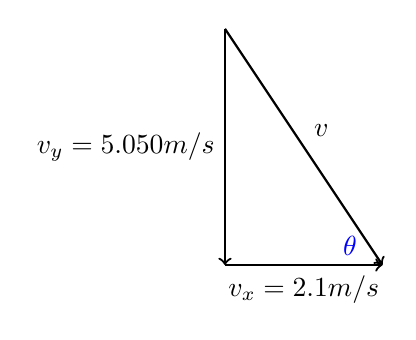
\begin{tikzpicture}
		% Draw the vertical side (v_x)
		\draw[->, thick] (0,0) -- (0,-3) node[midway, left] {$v_y = \SI{5.050}{m/s}$};
		
		% Draw the horizontal side (v_y)
		\draw[->, thick] (0,-3) -- (2,-3) node[midway, below] {$v_x = \SI{2.1}{m/s}$};
		
		% Draw the hypotenuse (v)
		\draw[->, thick] (0,0) -- (2,-3) node[midway, above right] {$v$};
		
		\node at (1.8,-3) [above left,blue] {$\theta$};
		
	\end{tikzpicture}

		Using the pythagorean theorum, we find:
			\begin{equation*}
			v = \sqrt{v_x^2 + v_y^2} = \sqrt{(\SI{2.1}{m/s})^2+(\SI{5.050}{m/s})^2} \approx \SI{5.470}{m/s}
		\end{equation*}
	
	\item The angle of impact is marked as \color{blue} $\theta$ \color{black} in the diagram for part 3.  We can find the angle of impact by using trigonometry.  Using tangent yields:
	
			\begin{equation*}
	\tan {\theta} = \frac{opp}{adj} 
	\end{equation*}

	\begin{equation*}
	\theta = \tan^{-1} (\frac{opp}{adj}) = \tan^{-1} (\frac{v_y}{v_x}) = \tan^{-1} (\frac{\SI{5.050}{m/s}}{\SI{2.1}{m/s}}) \approx 67.420 \degree
	\end{equation*}

		
	\end{enumerate}

	
\end{mdframed}	
	
	
	
	
	
	\subsection{Projectiles Launched at an Arbitrary Angle}
	\index{Projectiles, Launched at an Arbitrary Angle}
	
	When projectiles are launched at an angle, the initial horizontal and vertical components of the initial velocity can be determined using trigonometry.  
	\begin{figure}[h]
		\begin{center}	

	\begin{tikzpicture}[>=Stealth, thick, x=1cm, y=1cm]
		
		% Parameters
		\def\ang{32}     % <-- angle theta (degrees)
		\def\R{4}        % <-- length of v0 (arbitrary units)
		
		% Coordinates
		\coordinate (O) at (0,0);
		\coordinate (V) at (\ang:\R);                 % tip of v0
	\path (V -| O) coordinate (Xc);   % same x as V, y = 0
	\path (V |- O) coordinate (Yc);   % x = 0, same y as V
	
		\coordinate (Ex) at (1,0);                    % point on +x for angle pic
		
		% Axes
		\draw[->] (-0.5,0) -- (5.2,0) node[below right] {$x$};
		\draw[->] (0,-0.5) -- (0,4.2) node[above left] {$y$};
		
		% Resultant vector v0
		\draw[->,very thick] (O) -- (V) node[above right=2pt] {$\vec v_0$};
		
		% Components
		\draw[->,very thick,blue] (3.392,0) -- (3.392,2.12) node[below right=2pt] {$v_{0y}=v_0\sin\theta$};
		\draw[->,very thick,red]  (O) -- (Yc) node[below left=2pt] {$v_{0x}=v_0\cos\theta$};
		
		% Projection guides (dashed)
		\draw[dashed] (V) -- (Xc);
		\draw[dashed] (V) -- (Yc);
		
		% Angle theta at the origin
		\pic[draw,->,"$\theta$",angle eccentricity=1.3,angle radius=1.0cm]
		{angle=Ex--O--V};
		
		% Right-angle corner marker at the projection
		\draw ($(Xc)+(0,0)$) -- ++(0,0.25) -- ++(0.25,0);
	\end{tikzpicture}
\caption{The horizontal And vertical components of initial velocity.}
\label{Figure:vocomponents}
\end{center}
	\end{figure}

	In general, when the angle of elevation from horizontal is provided, as shown in Figure \ref{Figure:vocomponents}, the following equations allow you to deterine the initial and horizontal components of the initial velocity:
	
	\index{Inital Velocity, Components}
	\begin{equation}
		\overrightarrow{v_{ox}} = \overrightarrow{v_o} \cos \theta
	\end{equation}
	
		\begin{equation}
		\overrightarrow{v_{oy}} = \overrightarrow{v_o} \sin \theta
	\end{equation}

You can then solve the problem using normal kinematic equations.  

\begin{mdframed}[backgroundcolor=blue!10!white]
	\begin{center}
		
		
		\textbf{Example \thesection.1}	
	\end{center}
	
	\textbf{Problem: } A cannon launches a cannonball into the air with an initial speed of 125 m/s at an angle of 32 degrees above horizontal.  
	\begin{enumerate}
		\item How long does the cannonball take to get to the top of its path?
		\item How high does the cannonball go?
		\item How far does the cannonball land from its launchpoint?
	\end{enumerate}
	\vspace{0.1in}
	
	\textbf{Solution:} 
	Begin by drawing a diagram:
\begin{center}
	
\begin{tikzpicture}[>=Stealth, thick, scale=0.4]
	
	% Origin
	\coordinate (O) at (0,0);
	\coordinate (Xaxis) at (10,0);   % point on x-axis for angle marker
	\coordinate (Dir) at (8,6);      % direction of launch for angle marker
	
	% Launch vector
	\draw[->,very thick,blue] (O) -- (8,6) node[above right] {$\vec v_0$};
	

	
	% Dotted parabolic trajectory (manually chosen coefficients)
	\draw[densely dotted,very thick,domain=0:24,samples=60,smooth,variable=\x]
	plot ({\x},{0.5*\x - 0.02*\x*\x});
	
	% Reference point on trajectory
	\coordinate (P) at (12,{0.5*12 - 0.02*12*12}); % (12,3.12)
	
	% Horizontal guide (x - x0)
	\draw[decorate,decoration={brace,amplitude=6pt,mirror}]
	(O) -- (24,0) node[midway,below=6pt] {$x - x_0$};
	
	% Vertical guide (y - y0)
	\draw[decorate,decoration={brace,amplitude=6pt,mirror}]
	(24.5,0) -- (24,3.12) node[midway,right=6pt] {$y - y_0$};
	
	% Mark the point
	\fill (P) circle (2pt);
	
\end{tikzpicture}

\end{center}



\begin{enumerate}
	\item To find the time it takes to get to the top, we will us the rising portion of the motion only.  We can find the initial x- and y- component velocities by using trigonometry:
	
		\begin{equation*}
		\overrightarrow{v_{ox}} = \overrightarrow{v_o} \cos \theta = (\SI{125}{m/s}) \cos(32\deg) \approx \SI{106.006}{m/s}
	\end{equation*}
	
	\begin{equation*}
		\overrightarrow{v_{oy}} = \overrightarrow{v_o} \sin \theta = (\SI{125}{m/s}) \sin(32 \deg) \approx \SI{66.240}{m/s}	
	\end{equation*}
	
	
	
	
	
	We know that at the top, the projectile's vertical velocity will be zero, so we can write the following variables:
	
		
	\begin{longtable}{|c l | c l|}
		\hline
		\multicolumn{2}{|c|}{\textbf{Horizontal}} & \multicolumn{2}{|c|}{\textbf{ Vertical}} \\
		\hline
		$\vec{x}-\vec{x_0}$ =&     & $\vec{y}-\vec{y_0} = $ &   \\
		\hline
		$\vec{v_{0x}} = $ & $\SI{106.006}{m/s}$ & $\vec{v_{0y}} = $ & $\SI{66.240}{m/s}$ \\
		\hline
		$v_x = $&  & $v_y = $ & \SI{0}{m/s} \\
		\hline
		$a_x = $ & $\SI{0}{m/s^2}$ & $a_y = $ & $\SI{-9.81}{m/s^2}$ \\ 
		\hline
		\multicolumn{2}{|r}{$t = $} & \multicolumn{2}{l|}{  }  \\
		\hline
	\end{longtable}
	
	
	We can now calculate the time to the top by using equation \ref{equation:kinematic2} in the y-direction:
	
	\begin{equation*}
	\overrightarrow{v_y} = \overrightarrow{v_{0y}} + \overrightarrow{a_y} t \longrightarrow t = \frac{\overrightarrow{v_y}-\overrightarrow{v_{oy}}}{\overrightarrow{a_y}} = \frac{\SI{0}{m/s}-\SI{66.240}{m/s}}{\SI{-9.81}{m/s^2}} \approx \SI{6.752}{s}
	\end{equation*}	

\item We can now calculate the maximum height, $\overrightarrow{y}-\overrightarrow{y_0}$  by using any of equations \ref{equation:kinematic1}, \ref{equation:kinematic3}, or \ref{equation:kinematic4} in the y-direction.  While all of these equations will yield the same result, in order to minimize rounding error, the author chooses equation \ref{equation:kinematic4} in this situation.  

\begin{equation*}
	\overrightarrow{v_y}^2 = \overrightarrow{v_{0y}}^2 + 2\overrightarrow{a_y}(\overrightarrow{y}-\overrightarrow{y_0}) \longrightarrow 	\overrightarrow{y}-\overrightarrow{y_0} = \frac{\overrightarrow{v_y}^2 -\overrightarrow{v_{0y}}^2 }{2\overrightarrow{a_y}}
\end{equation*}

\begin{equation*}
	\overrightarrow{y}-\overrightarrow{y_0} = \frac{(\SI{0}{m/s})^2 -(\SI{66.240}{m/s})^2 }{2(\SI{-9.81}{m/s^2})} \approx \SI{223.635}{m}
\end{equation*}
	
	\item It should be noted that the time calculated in part (1) of this problem is the time it takes for the ball to reach its highest point - which is when the ball has only traveled half its horizontal distance.  Due to the symmetry of the situation, we can double the time to find the total time of flight.  This can be used to calculate the distance the ball travels in the x- direction.
	
	\begin{equation}
		t_{total} = 2 t_{rising} = 2 \times \SI{6.752}{s} \approx \SI{13.505}{s}
	\end{equation}
	
	Using equation \ref{equation:kinematic3} in the x-direction gives:	
		\begin{equation}
		\overrightarrow{x}-\overrightarrow{x_0} = \overrightarrow{v_0} t + \cancelto{0}{\frac{1}{2}\vec{a}{t}^2} =  \overrightarrow{v_0} t = (\SI{106.006}{m/s})(\SI{13.505}{s}) \approx \SI{1431.565}{m}
	\end{equation}
\end{enumerate}
	
\end{mdframed}	

		


	


